\subchapter{Using the I2C bus}{Objective: make the I2C bus work and
use it to implement communication with the Nunchuk device}

After this lab, you will be able to:

\begin{itemize}
\item Declare pinctrl settings.
\item Access I2C device registers through the bus.
\end{itemize}

\section{Setup}

Stay in the \code{~/linux-kernel-labs/src/linux} directory for kernel and DTB
compiling (stay in the \code{nunchuk} branch), and in
\code{~/linux-kernel-labs/modules/nfsroot/root/nunchuk} for module compiling
(use two different terminals).

\section{Remove debugging messages}

Now that we have checked that the \code{probe()} and \code{remove()} functions
are called, remove the \kfunc{pr_info} messages that you added to
trace the execution of these functions.

\section{Connecting the nunchuk}

Take the nunchuk device provided by your instructor.

We will connect it to the second I2C port of the CPU (\code{i2c1}),
which pins are available on the \code{P9} connector.

Now we can identify the 4 pins of the nunchuk connector:

\begin{center}
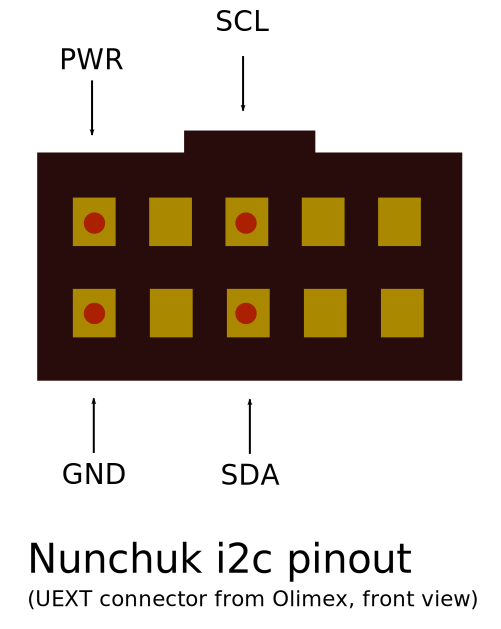
\includegraphics[width=4cm]{common/nunchuk-pinout.pdf}
\end{center}

Open the System Reference Manual that you downloaded earlier,
and look for "connector P9" in the table of contents, and then
follow the link to the corresponding section. Look at the table listing
the pinout of the P9 connector.

Now connect the nunchuk pins:
\begin{itemize}
\item The \code{GND} pin to P9 pins 1 or 2 (\code{GND})
\item The \code{PWR} pin to P9 pins 3 or 4 (\code{DC_3.3V})
\item The \code{SCL} pin to P9 pin 17 (\code{I2C1_SCL})
\item The \code{SDA} pin to P9 pin 18 (\code{I2C1_SDA})
\end{itemize}

\begin{center}
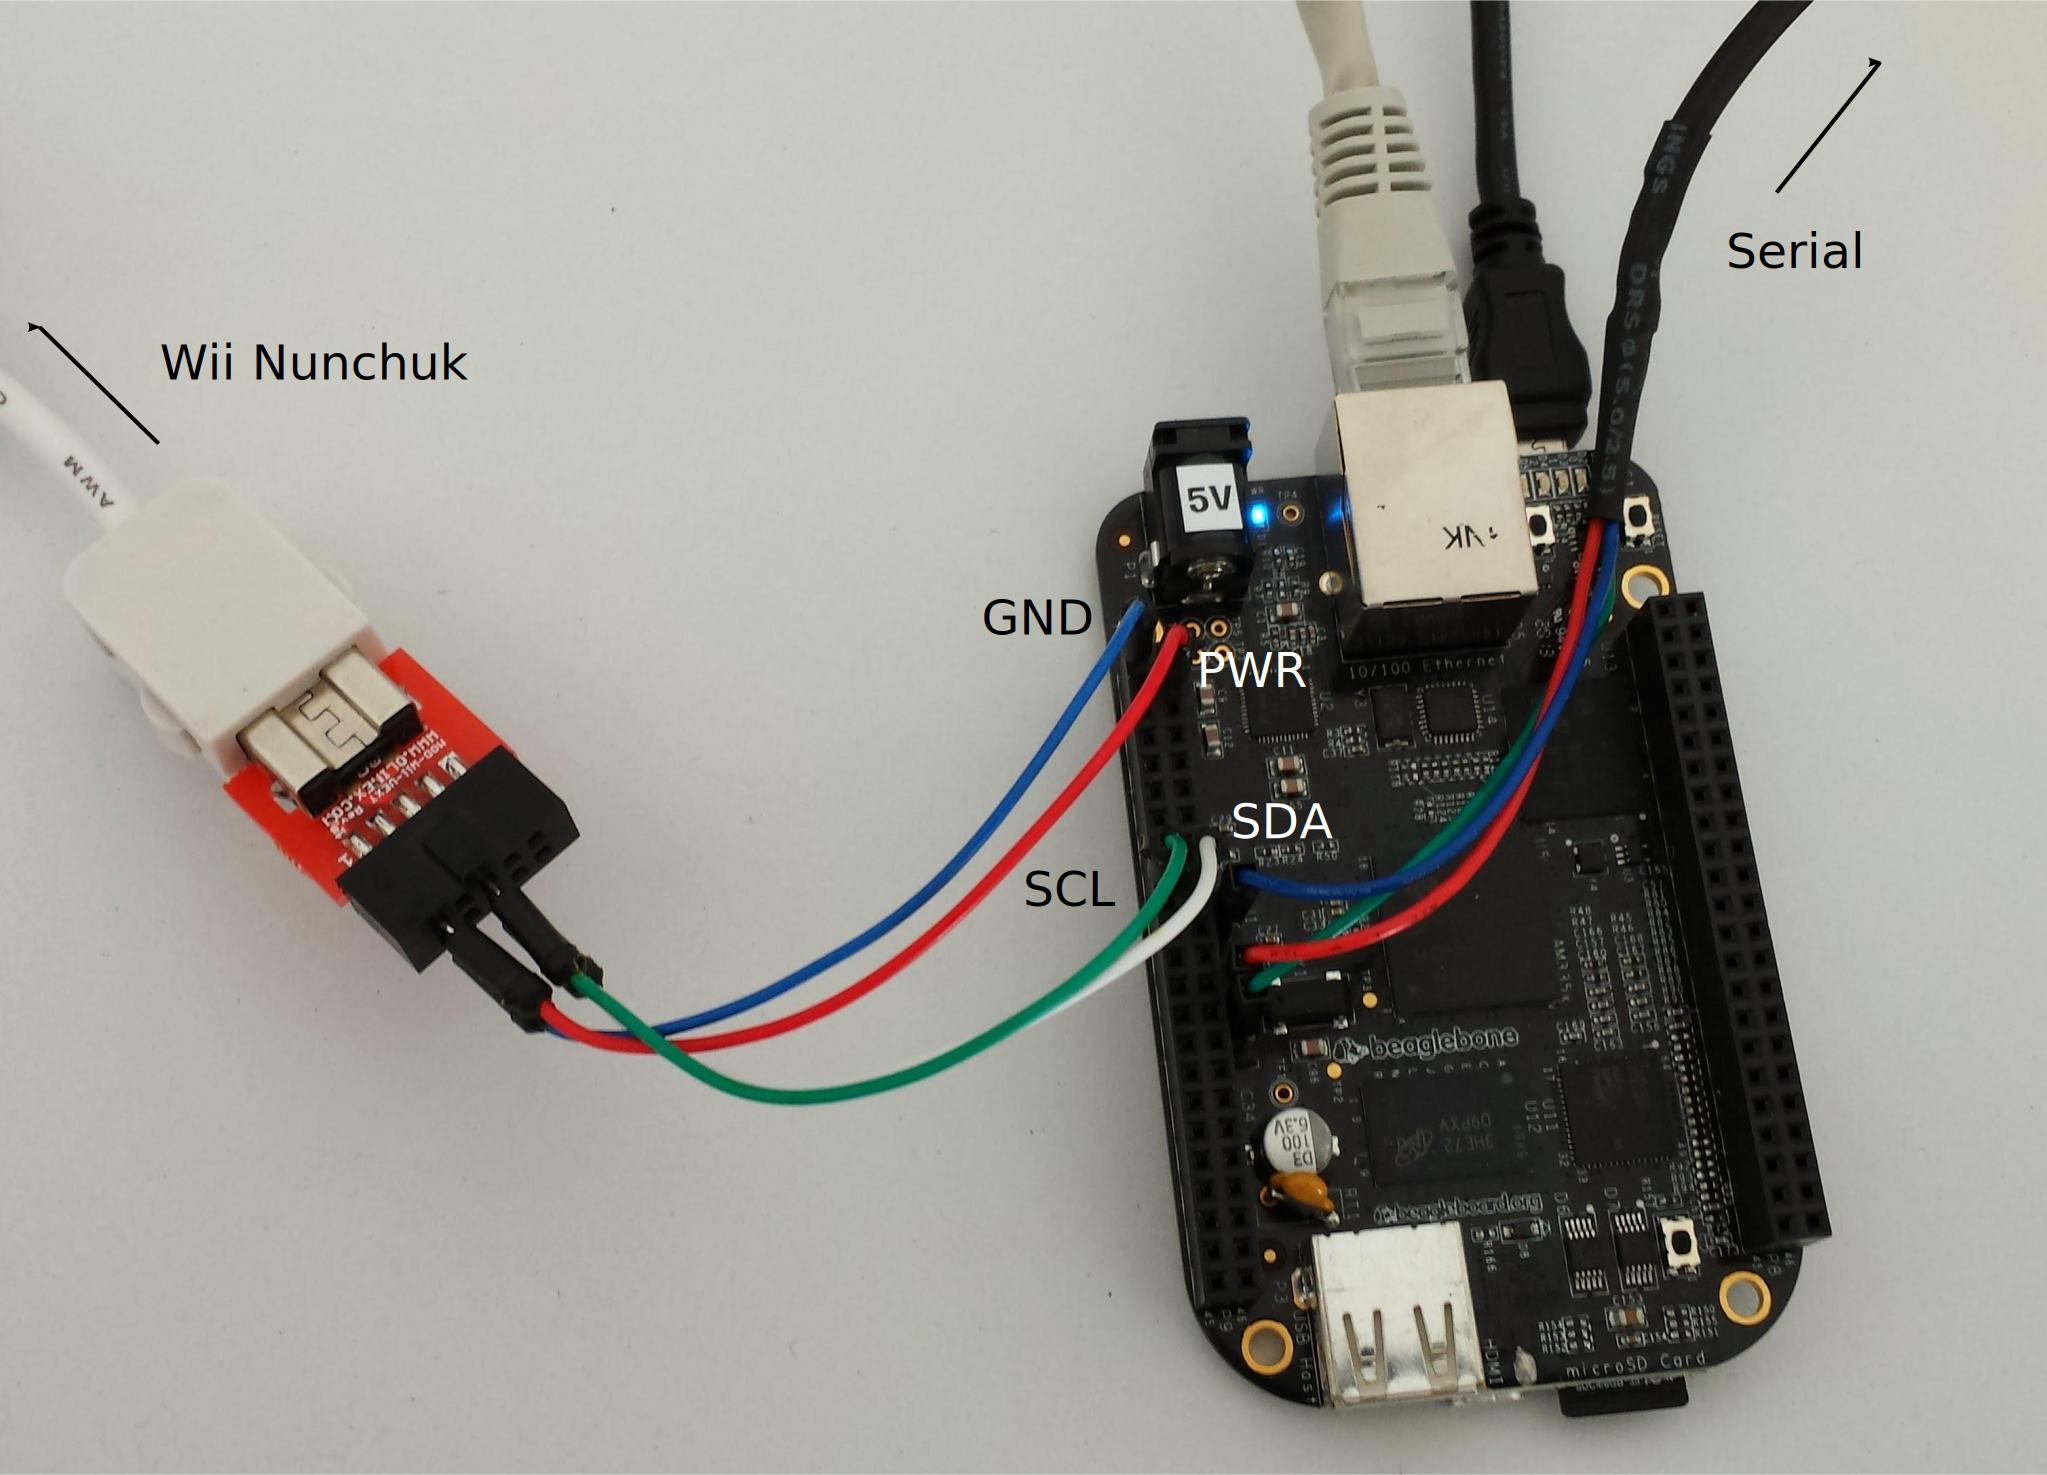
\includegraphics[width=12cm]{common/bbb-connect-nunchuk.pdf}
\end{center}

\section{Find pin muxing configuration information for i2c1}

As you found in the previous lab, we now managed to have our nunchuk
device enumerated on the \code{i2c1} bus.

However, to access the bus data and clock signals, we need to configure
the pin muxing of the SoC.

If you go back to the BeagleBone Black System Reference Manual, in the
{\em Connector P9} section, you can see that the pins \code{17} and
\code{18} that we are using correspond to pins \code{A16} and \code{B16}
of the AM335 SoC. You can also see that such pins need to be configured
as \code{MODE2} to get the functionality that we need (\code{I2C1_SCL}
and \code{I2C1_SDA}).

The second step is to open the CPU datasheet (\code{am3359.pdf}), and
look for pin assignment information ({\em Pin Assignments} section).
You will find that the processor is available through two types of
packages: \code{ZCE} and \code{ZCZ}. If you have an original
BeagleBoneBlack board, you can have a very close look at the CPU
(with your glasses on!) and you will see that the CPU has \code{ZCZ} written
on its lower right corner. On BeagleBoneBlack Wireless with the
Octavo System In Package, you can no longer find such information.
Anyway, the \code{ZCZ} package information applies to both types of
boards.

So, in the {\em ZCZ Package Pin Maps (Top View)} section\footnote{Caution: you
won't be able to search the PDF file for this section name, for obscure
reasons. At the time of this writing, this section is numbered 4.1.2.}, you can find
hyperlinks to the descriptions of the \code{A16} and \code{B16} pins.
That's where you can find reference pin muxing information for these
pins.  You can find that the pin name for \code{A16} is \code{SPI0_CS0}
and that the pin name for \code{B16} is \code{SPI0_D1}.
You can also get confirmation that to obtain the (\code{I2C1_SCL} and
\code{I2C1_SDA}) signals, you need to configure muxing mode number 2.
You can also see that both pins support pull-up and pull-down
modes\footnote{See \url{https://en.wikipedia.org/wiki/Pull-up_resistor}}
(see the \code{PULLUP /DOWN TYPE} column).

The next thing to do is to open the big TRM document and look for the
address of the registers that control pin muxing. First, look for
{\em L4\_WKUP Peripheral Memory Map} with your PDF reader search
utility. You will find a table containing a
\code{Control Module Registers} entry with its address:
\code{0x44E1_0000}.

Last but not least, look for the \code{SPI0_CS0} and \code{SPI0_D1}
pin names, and you will find the offsets for the registers controlling
muxing for these pins in the {\em CONTROL\_MODULE REGISTERS} table:
respectively \code{0x95c} and \code{0x958}.

We now know which registers we can write to to enable \code{i2c1}
signals.

\section{Add pinctrl properties to the Device Tree}

Now that we know the register offsets, let's try to understand
how they are used in existing code. For example, open the
the Device Tree for the AM335x EVM board
(\kfile{arch/arm/boot/dts/am335x-evm.dts}), which is using
\code{i2c1} too. Look for \code{i2c1_pins}, and you will see how
offsets are declared and what values they are given:

{\small
\begin{verbatim}
i2c1_pins: pinmux_i2c1_pins {
	pinctrl-single,pins = <
		AM33XX_PADCONF(AM335X_PIN_SPI0_D1, PIN_INPUT_PULLUP, MUX_MODE2)	/* spi0_d1.i2c1_sda */
		AM33XX_PADCONF(AM335X_PIN_SPI0_CS0, PIN_INPUT_PULLUP, MUX_MODE2)	/* spi0_cs0.i2c1_scl */
	>;
};
\end{verbatim}
}

Here are details about the values:

\begin{itemize}
\item \ksym{AM335X_PIN_SPI0_D1} and \ksym{AM335X_PIN_SPI0_CS0} offsets
      in the Pin Controller registers to control muxing on the
      corresponding package pins.
\item \ksym{MUX_MODE2} corresponds to muxing mode 2, as explained in the
      datasheet.
\item \ksym{PIN_INPUT_PULLUP} puts the pin in pull-up mode (remember
      that our pins support both pull-up and pull-down). It seems to
      be needed for I2C bus operation.
\end{itemize}

Now that pin muxing settings have been explained, edit your board
DTS file to add the same definitions to enable pin muxing for \code{i2c1}.
Don't forget that you don't have to repeat definitions that are
already present in the \code{.dtsi} files. Just add new declarations, or
settings that override common definitions.

Rebuild and update your DTB, and eventually reboot the board.

\section{I2C bus tests}

We will use the \code{i2cdetect} command to make sure that
everything works fine for \code{i2c1}:

\begin{verbatim}
# i2cdetect -l
i2c-0	i2c       	OMAP I2C adapter                	I2C adapter
i2c-2	i2c       	OMAP I2C adapter                	I2C adapter
i2c-1	i2c       	OMAP I2C adapter                	I2C adapter
\end{verbatim}

\begin{verbatim}
# i2cdetect -F 1
Functionalities implemented by /dev/i2c-1:
I2C                              yes
SMBus Quick Command              no
SMBus Send Byte                  yes
SMBus Receive Byte               yes
SMBus Write Byte                 yes
SMBus Read Byte                  yes
SMBus Write Word                 yes
SMBus Read Word                  yes
SMBus Process Call               yes
SMBus Block Write                yes
SMBus Block Read                 no
SMBus Block Process Call         no
SMBus PEC                        yes
I2C Block Write                  yes
I2C Block Read                   yes
\end{verbatim}

You can see that the {\em SMBus Quick Commands} are not available on
this driver, yet \code{i2cdetect} uses them by default to scan the i2c
bus. You can use \code{i2cdetect -r} to use the usual set of i2c
commands, and be able to detect the devices on your bus.

To test if everything works fine, run \code{i2cdetect -r 1}. This will
scan the \code{i2c1} bus for devices. You should see a device at the
address \code{0x52}. This is your nunchuk.

If everything works as expected, commit your Device Tree changes. This
will be required to switch to another branch later:

\begin{verbatim}
git commit -as
\end{verbatim}

\begin{itemize}
\item \code{git commit -a} adds all the files already known to
      \code{git} to the commit.
\item \code{git commit -s} adds a \code{Signed-off-by} line (required
      for all contributions to the Linux kernel).
\end{itemize}

\section{Device initialization}

The next step is to read the state of the nunchuk registers, to find out
whether buttons are pressed or not, for example.

Before being able to read nunchuk registers, the first thing to do is
to send initialization commands to it. That's also a nice way of making
sure i2c communication works as expected.

In the probe routine (run every time a matching device is found):

\begin{enumerate}
\item Using the I2C raw API (\kfunc{i2c_master_send} and
        \kfunc{i2c_master_recv}), send two bytes to the
        device: \code{0xf0} and \code{0x55}\footnote{
	The I2C messages to communicate with a wiimote
        extension are in the form: \code{<i2c_address> <register> }
        for reading and \code{<i2c_address> <register> <value>} for
        writing. The address, \code{0x52} is sent by the i2c framework
        so you only have to write the other bytes, the register
        address and if needed, the value you want to write. There are
        two ways to set up the communication. The first known way was
        with data encryption by writing \code{0x00} to register
        \code{0x40} of the nunchuk.  With this way, you have to
        decrypt each byte you read from the nunchuk (not so hard but
        something you have to do).  Unfortunately, such encryption
        doesn't work on third party nunchuks so you have to set up
        unencrypted communication by writing \code{0x55} to
        \code{0xf0} instead. This works across all brands of nunchuks
        (including Nintendo ones).}.
      Make sure you check the return value of the function you're
      using. This could reveal communication issues.  Using Elixir, find
      examples of how to handle failures properly using the same
      function.

\item Let the CPU wait for 1 ms by using the \kfunc{udelay} routine.
      Let's use Elixir again to find the right C headers to include...

      The Elixir results are a bit confusing here, because
      \kfunc{udelay} is defined in \code{arch/<arch>/include/asm/delay.h} files,
      but not in an \code{include/linux/<file>.h>} that is normally used
      in kernel code.

      However, look at \kfile{include/linux/delay.h} and you will see
      that it includes \code{asm/delay.h} which corresponds to the
      specific headers for the current architecture. So you need to include
      \code{linux/delay.h}.

      {\bf General rule}: whenever the symbol you're looking
      for is defined in \code{arch/<arch>/include/asm/<file>.h}, you
      can include \code{linux/<file>.h} in your kernel code.

\item In the same way, send the \code{0xfb} and \code{0x00} bytes now.
      This completes the nunchuk initialization.
\end{enumerate}

Recompile and load the driver, and make sure you have no communication
errors.

\section{Read nunchuk registers}

The nunchuk exhibits a rather weird behavior: it seems that it updates
the state of its internal registers only when they have been read.

As a consequence, we will need to read the registers twice!

To keep the code simple and readable, let's create a
\code{nunchuk_read_registers} function to read the registers once.
In this function:

\begin{enumerate}
\item Start by putting a \code{10 ms} delay by calling
      \code{usleep_range(10000, 20000)}, guaranteed to sleep between 10 and 20
      ms.\footnote{That's better than using \kfunc{udelay} because it is not making
      an active wait, and instead lets the CPU run other tasks in the meantime.
      You'll find interesting details on how to sleep or wait in kernel
      code for specified durations in the kernel documentation:
      \kerneldochtml{timers/timers-howto}.}
      Such waiting time is needed to add time between the previous i2c
      operation and the next one.
\item Write \code{0x00} to the bus. That will allow us to read
      the device registers.
\item Add another \code{10 ms} delay.
\item Read 6 bytes from the device, still using the I2C raw API.
      Check the return value as usual.
\end{enumerate}

\section{Reading the state of the nunchuk buttons}

Back to the \code{probe()} function, call your new function twice.

After the second call, compute the states of the \code{Z} and \code{C}
buttons, which can be found in the sixth byte that you read.

As explained on
\url{https://bootlin.com/labs/doc/nunchuk.pdf}:

\begin{itemize}
\item \code{bit 0 == 0} means that \code{Z} is pressed.
\item \code{bit 0 == 1} means that \code{Z} is released.
\item \code{bit 1 == 0} means that \code{C} is pressed.
\item \code{bit 1 == 1} means that \code{C} is released.
\end{itemize}

Using boolean operators, write code that initializes a \code{zpressed}
integer variable, which value is \code{1} when the \code{Z} button is
pressed, and \code{0} otherwise. Create a similar \code{cpressed}
variable for the \code{C} button\footnote{You may use the \kfunc{BIT}
macro, which will make your life easier. See Elixir for details.}.

The last thing is to test the states of these new variables at the end
of the \code{probe()} function, and log a message to the console
when one of the buttons is pressed.

\section{Testing}

Compile your module, and reload it. No button presses should be
detected. Remove your module.

Now hold the \code{Z} button and reload and remove your module again:
\begin{verbatim}
insmod /root/nunchuk/nunchuk.ko; rmmod nunchuk
\end{verbatim}

You should now see the message confirming that the driver found
out that the \code{Z} button was held.

Do the same over and over again with various button states.

At this stage, we just made sure that we could read the state
of the device registers through the I2C bus. Of course, loading and
removing the module every time is not an acceptable way of
accessing such data. We will give the driver a proper {\em input}
interface in the next slides.
